\section{Analizador Vectorial de Redes}
El Analizador Vectorial de Redes fue definido en sus inicios como un instrumento que permite medir los parámetros de redes eléctricas \cite{Tektronix}. En su esquema más básico posee una fuente de radiofrecuencias (RF), que genera una señal de estímulo para el dispositivo bajo prueba, y un banco de receptores que miden las señales que salen del DUT y las comparan con la onda incidente. Los resultados se procesan y muestran al usuario por medio de alguna interfaz.

Dependiendo de los dispositivos que se buscan caracterizar, se determina la cantidad de puertos que debe tener el VNA. Un puerto permite medir el parámetro de reflexión. Con dos puertos, se puede medir además el de transmisión. Si posee un solo canal, se puede medir la transmisión inversa y la reflexión en la salida invirtiendo físicamente el dispositivo bajo prueba. Este paso se puede evitar agregando un canal, lo que incrementa el costo del VNA.

Impedancia de entrada/S11 

\section{Parámetros distribuidos (S)}
Los parámetros distribuidos, también llamados S por su nombre en inglés (\textit{Scattering}) permiten caracterizar redes de dos o más puertos en función de sus ondas entrantes y salientes. Se especifican para una impedancia de referencia y a una frecuencia específica, y son útiles en altas frecuencias porque otros tipos de parámetros (como los Z o los Y) no pueden ser medidos directamente.  

 \begin{figure}[H]
    \centering
    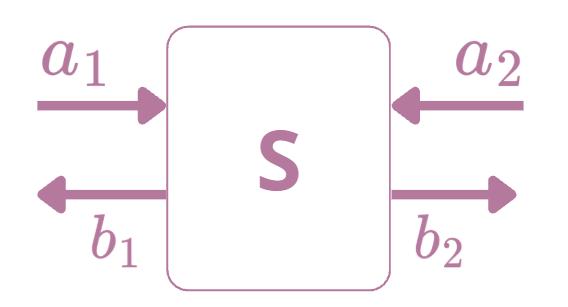
\includegraphics[trim={0 0cm 0.0cm  0 0cm},clip,width=6cm]{Imagenes/par_S.png}
    \caption{Parámetros S}
    \label{parS}
 \end{figure}

Según las ondas incidentes $a_{1}$ y $a_{2}$ y las reflejadas $b_{1}$ y $b_{2}$, los parámetros S se definen como:
\\

$S_{11} = \left. \frac{b_1}{a_1} \right|_{a_2=0}$; $S_{12} = \left. \frac{b_1}{a_2} \right|_{a_1=0}$; $S_{21} = \left. \frac{b_2}{a_1} \right|_{a_2=0}$; $S_{22} = \left. \frac{b_2}{a_2} \right|_{a_1=0}$
\\

Para lograr que las $a$ sean iguales a 0, el puerto al que pertenecen debe estar adaptado, garantizando que no haya ninguna señal incidente. El parámetro $S_{11}$ se conoce como el coeficiente de reflexión en el puerto 1 cuando el puerto 2 está adaptado.

\section{Calibración}
\subsection{Errores}
Los errores que pueden aparecer en una medición se pueden dividir en dos grandes clases: los errores sistemáticos y los aleatorios. Los primeros se pueden corregir, mientras que los segundos se encuentran en toda medición y están fuera del control del usuario.

En el caso de dispositivos electrónicos algunos errores sitemáticos son los producidos por variaciones en la potencia de salida de los generadores, pérdidas de inserción en materiales conductores y conectores, desfasajes ocasionados por diferencias en longitudes eléctricos o retardos en los circuitos integrados, reflexiones generadas por desadaptación de impedancias y deriva térmica. Algunos errores aleatorios pueden ser ruido térmico, de cuantización e interferencia electromagnética.

La calibración en un VNA permite corregir los errores sistemáticos, excluyendo el ruido por deriva térmica. Este se puede corregir solo si la calibración se realiza inmediatamente antes de la medición.

\subsection{Método SOL}
En VNAs de un puerto se pueden simplificar los errores a un modelo de tres términos que describen la directividad, adaptación del puerto y errores de seguimiento (variaciones de amplitud y fase en función de la frecuencia)\cite{Rytting}. Usando tres cargas distintas de valores conocidos, se puede formar un sistema de tres ecuaciones con tres incógnitas y resolver para obtener los términos del error:

\begin{subequations}\label{eq:sistema_calibracion}
\begin{align}
    e_{00} + \Gamma_1 \Gamma_{\text{M}1} e_{11} - \Gamma_1 \Delta_e &= \Gamma_{\text{M}1} \label{eq:calib1} \\
    e_{00} + \Gamma_2 \Gamma_{\text{M}2} e_{11} - \Gamma_2 \Delta_e &= \Gamma_{\text{M}2} \label{eq:calib2} \\
    e_{00} + \Gamma_3 \Gamma_{\text{M}3} e_{11} - \Gamma_3 \Delta_e &= \Gamma_{\text{M}3} \label{eq:calib3}
\end{align}
\end{subequations}

Donde $\Gamma_{\text{M}}$ es el parámetro de reflexión medido para cada carga, y $\Delta_e=e_{00}e_{11}-(e_{10}e_{01})$. Los términos del error se pueden observar en la figura \ref{errorescalibracion}. 

 \begin{figure}[H]
    \centering
    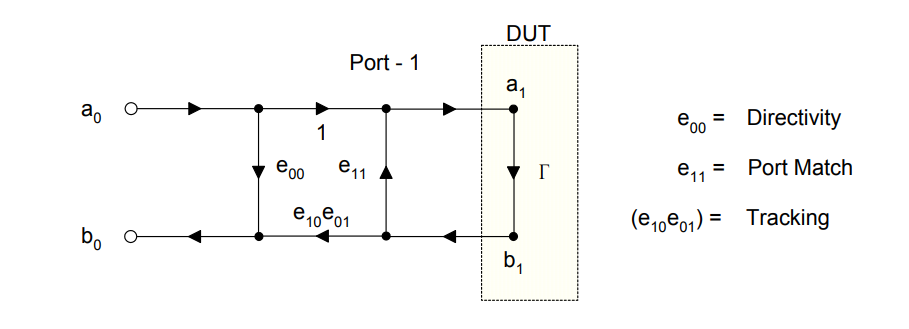
\includegraphics[trim={0 0cm 0.0cm  0 0cm},clip,width=\linewidth]{Imagenes/errorescalibracion.png}
    \caption{Términos de error para un VNA de un puerto}
    \label{errorescalibracion}
 \end{figure}

Si las cargas independientes son un circuito abierto, cortocircuito y carga de 50$\Omega$ entonces el método de calibración se denomina SOL (Short, Open, Load) y las ecuaciones \eqref{eq:sistema_calibracion} se simplifican a:

\begin{subequations}\label{eq:sistema_SOL}
\begin{align}
    e_{00} - \Gamma_{\text{MS}} e_{11} + \Delta_e &= \Gamma_{\text{MS}} \label{eq:sol_s} \\
    e_{00} + \Gamma_{\text{MO}} e_{11} - \Delta_e &= \Gamma_{\text{MO}} \label{eq:sol_o} \\
    e_{00} &= \Gamma_{\text{ML}} \label{eq:sol_l}
\end{align}
\end{subequations}

Luego el $\Gamma$ real se calcula como:

\begin{equation}
    \Gamma= \frac{\Gamma_{M}-e_{00}}{\Gamma_{M}e_{11}-\Delta_{e}}
\end{equation}

 
\section{Acoplador Direccional}
En la mayoría de diseños en electrónica, el acoplamiento electromagnético entre líneas de transmisión se considera ruido porque interfiere con la señal que se busca transmitir. Una excepción es el caso de acopladores, donde el acoplamiento es un parámetro de diseño que permite medir la señal de una línea con un alto aislamiento, es decir, sin interrumpir su paso. Además cuando se dispone de un par de lineas acopladas, se puede verificar que en uno de sus puertos la señal incidente se anula, generando un punto que permite medir la onda reflejada. 

Las principales propiedades que caracterizan un acoplador son la directividad, el aislamiento, el acoplamiento y la pérdida de inserción \cite{acopladores_minicircuits}. La directividad mide la capacidad de separar las ondas que se propagan en distintas direcciones. El aislamiento, la potencia que llega a la carga desacoplada. El acoplamiento indica la potencia que se entrega al puerto acoplado. La pérdida de inserción tiene en cuenta cuánta potencia que se debería transmitir se pierde por ser entregada a los puertos acoplados y aislados, y tiene en cuenta las pérdidas en los materiales (dieléctrico y resistividad de las pistas). 

Un acoplador ideal es un dispositivo pasivo, que posee directividad y aislamiento infinitos. 

Existen acopladores direccionales como el HP 778d \cite{keysight_778d} que posee una directividad mayor a 36dB y pérdidas por inserción menores a 0,6dB, pero tiene un ancho de banda que permite hacer mediciones entre 100 MHz y 2 GHz, y sus dimensiones físicas y peso hacen que su utilidad se limite a mediciones en laboratorio. Para soluciones integradas hay alternativas comerciales como el ZABDC20-322 de Minicircuits \cite{minicircuits_zabdc20} pero su costo hace que el diseño no sea escalable. 

\subsection{Puente resistivo}
Una solución compacta, económica y con un ancho de banda teórico infinito es el puente resistivo tipo Wheatstone. Como se puede observar en la figura \ref{fig:puente_wheatstone} es una red simple de comparación de impedancias, formada por cuatro resistencias sobre las cuales se inyecta una señal de referencia en la parte superior. Una de las resistencias es variable (Zx), mientras que el resto son iguales entre sí. Se utiliza un voltímetro para medir la diferencia de potencial entre las ramas. Si la resistencia variable es de 50$\Omega$, el puente queda balanceado y el voltímetro indica un cero. Si es menor a 50$\Omega$, la rama izquierda presenta un voltaje menor a la derecha, mientras que para valores mayores ocurre lo opuesto.  Si la señal incidente es sinusoidal es posible además caracterizar cargas reactivas midiendo el desfasaje de la señal Zx respecto de la incidente. Este es el principio que permite al puente comportarse como un acoplador direccional: la diferencia de potencial entre las ramas es función de la onda reflejada equivalente.  

\begin{figure}
    \centering
    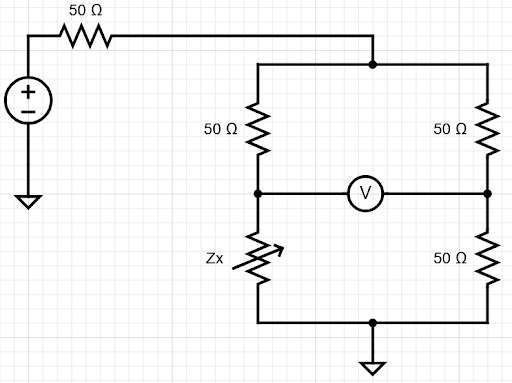
\includegraphics[width=0.5\linewidth]{Imagenes/puente_wheatstone.png}
    \caption{Esquema básico de un puente de Wheatstone}
    \label{fig:puente_wheatstone}
\end{figure}

\section{Reglas de diseño en RF}
Al momento de rutear un PBC (\textit{Printed Circuit Board} - Placa de Circuito Impreso) se deben tener en consideración algunas buenas prácticas que ayudan a mantener la integridad de las señales, la impedancia de las líneas y evitar la interferencia electromagnética, sobre todo cuando se trabaja en RF. 

Se debe garantizar que las pistas cumplan con la impedancia requerida de 50$\Omega$. Esto implica calcular el ancho de la línea usando las ecuaciones de diseño según el tipo de línea o se pueden encontrar calculadoras online o integradas en los software de diseño con este fin. Se deben evitar ángulos rectos, que causan discontinuidades y aumentan la capacitancia parásita. 

El plano de masa que se encuentra debajo de las pistas de RF debe ser continuo, para que la corriente de retorno pueda seguir el camino de menor inductancia. Por esta razón no se recomienda rutear en el plano inferior al de las rutas de RF, pero si se necesita hacerlo no se deben atravesar las regiones donde en la capa superior haya trazos de RF.

Se deben usar las técnicas \textit{vía stitching} y \textit{vía shielding}. La segunda se usa para reducir la interferencia electromagnética y el crosstalk \cite{altium_via_stitching}, mientras que la primera "ata" los planos de masa de distintas capas, ayudando a mantener baja impedancia y caminos de retorno cortos. Además evita resonancias dentro de la placa.

Los capacitores de desacople se deben ubicar lo más cerca posible de los integrados, de forma de poder suministrar rápidamente los picos de corriente que demandan los integrados que la fuente de alimentación no puede entregar \cite{altium_caps_desacople}. También deben utilizarse cuando se suministra alimentación a un trazo a través de vías.

Los trazos deben ser lo más cortos posible, para minimizar la atenuación de las señales y reflexiones indeseadas.


\section{Heterodinación de señales}
Las señales que se intentan medir en un VNA son de naturaleza analógica, por lo que para realizar el cálculo del parámetro de reflexión o S11 primero se debe poder medir su amplitud y fase. Existen integrados que pueden obtener la magnitud de una onda de RF como el HMC601 \cite{AnalogDevices_HMC601} pero se pierde información de la fase. Por eso se busca una forma de bajar la frecuencia de la señal para poder adquirirla de forma digital.

Un esquema heterodino se basa en la combinación de una señal de RF de interés con otra señal generada localmente por un oscilador local (OL o LO por sus siglas en inglés) desplazada en frecuencia un valor constante, llamado frecuencia intermedia (FI). Es posible demostrar matemáticamente que cuando se multiplican idealmente en el dominio del tiempo dos señales sinusoidales, a la salida existen componentes espectrales en la suma y diferencia de las frecuencias originales. Mediante un filtrado se puede aislar la componente diferencia, logrando así trasladar la información de la señal de RF hacia la FI. 
Utilizando un mezclador doble se pueden heterodinar dos señales con un solo oscilador local, como muestra la figura \ref{fig:mixer} . De esta forma obtenienen las señales incidente y reflejada, conservando su amplitud y fase, en una frecuencia de audio que facilite su adquisición y procesamiento.

\begin{figure}
    \centering
    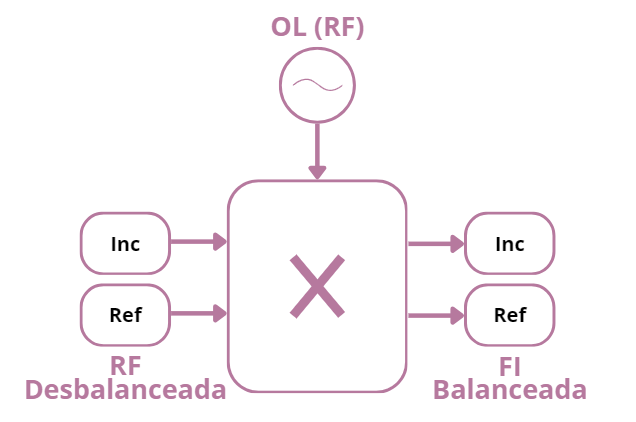
\includegraphics[width=0.5\linewidth]{Imagenes/mixer.png}
    \caption{heterodinación}
    \label{fig:mixer}
\end{figure}

\section{Procesamiento digital de señales}

Para poder aplicar un procesamiento digital cualquier señal analógica continua en el tiempo debe ser muestreada, es decir convertirla en una secuencia de números de precisión finita. El proceso implica una pérdida de información de los intervalos intermedios, pero según el teorema de Nyquist-Shannon una señal de banda limitada puede reconstruirse inequívocamente a partir de sus muestras si la frecuencia de muestreo $f_s$ cumple la condición $f_s \ge 2 f_{\max}$, donde $f_{\max}$ representa la componente frecuencial de mayor valor de la señal \cite{TDSmanolakis}.

Una vez que la señal está digitalizada, para poder extraer su amplitud y fase, sabiendo que se encuentra a una frecuencia de valor FI, se debe aplicar un filtrado digital y realizar la Transformada Rápida de Fourier (FFT - \textit{Fast Fourier Transform})


\subsection{Filtros digitales}
El objetivo principal de la etapa de filtrado es aislar la señal de FI eliminando el ruido de banda ancha, las interferencias de baja frecuencia y armónicos de orden superior. 

La señal muestreada $x[n]$ pasa por un filtro pasabanda digital caracterizado por una respuesta al impulso $h[n]$. La operación se define mediante la convolución discreta:
\begin{equation}
    y[n] = x[n] * h[n] = \sum_{k=0}^{M} h[k] \, x[n-k]
\end{equation}
donde $M$ representa el orden del filtro. Los coeficientes $h[k]$ se diseñan para configurar una banda de paso en torno a la frecuencia de FI.

Los filtros digitales se pueden clasificar en dos grandes familias según la naturaleza de su respuesta al impulso: filtros de respuesta finita (\textit{Finite Impulse Response}, FIR) y filtros de respuesta infinita (\textit{Infinite Impulse Response}, IIR).

Un filtro IIR se caracteriza por una respuesta al impulso de duración infinita, que se logra mediante una estructura recursiva con realimentación de las salidas anteriores. Su ecuación en diferencias se expresa como:
\begin{equation}
    y[n] = \sum_{k=0}^{M} b_k \, x[n-k] + \sum_{k=1}^{N} a_k \, y[n-k]
\end{equation}
La presencia de los coeficientes $a_k$ introduce polos en el plano z fuera del origen. Si bien permiten lograr bandas de transición abruptas con órdenes bajos, presentan dos desventajas fundamentales: no garantizan fase lineal en toda la banda de paso y pueden ser inestables si sus polos migran fuera del circulo unitario debido a cuantización de precisión finita.

Por otro lado, un filtro FIR presenta una respuesta al impulso de duración finita $N_{\text{taps}}$ (comúnmente denominada número de coeficientes o \textit{taps}), siendo $h[n] = 0$ para $n < 0$ y $n \ge N_{\text{taps}}$. Su ecuación en diferencias es puramente no recursiva:
\begin{equation}
    y[n] = \sum_{k=0}^{M} b_k \, x[n-k] = \sum_{k=0}^{N_{\text{taps}}-1} h[k] \, x[n-k]
\end{equation}
donde $M = N_{\text{taps}} - 1$ representa el orden del filtro. Su transferencia $H(z)$ es causal, estable y realizable. Todos sus polos se ubican de manera trivial en el origen ($z = 0$), lo que garantiza estabilidad incondicional.

Si la secuencia de coeficientes $h[n]$ cumple la condición de simetría par alrededor de su centro ($h[n] = h[N_{\text{taps}}-1-n]$), la respuesta en frecuencia presenta la forma:
\begin{equation}
    H(e^{j\omega}) = |H(e^{j\omega})| \, e^{-j \omega \tau_g}
\end{equation}
donde el retardo de grupo $\tau_g$ es estrictamente constante para todas las frecuencias:
\begin{equation}
    \tau_g = \frac{N_{\text{taps}} - 1}{2} \quad \text{[muestras]}
\end{equation}
Un retardo de grupo constante asegura que el filtro no introduce distorsión de fase no lineal, preservando la diferencia de fase relativa entre el canal de referencia ($V_{\text{ref}}$) y el de medición ($V_{\text{med}}$).

\subsubsection{Diseño de filtros FIR mediante el método del enventanado}

El diseño del filtro FIR se fundamenta en el método del enventanado (\textit{window design method}). Este método consiste en truncar y desplazar la respuesta al impulso ideal de duración infinita, $h_d[n]$ (correspondiente a un filtro pasabanda ideal centrado en $f_{\text{FI}}$), multiplicándola punto a punto por una función ventana finita $w[n]$ de longitud $N_{\text{taps}}$:
\begin{equation}
    h[n] = h_d[n] \cdot w[n], \quad 0 \le n \le N_{\text{taps}}-1
\end{equation}

Para la síntesis de la respuesta pasabanda se emplea la ventana de Hamming, definida analíticamente como:
\begin{equation}
    w[n] = 0{,}54 - 0{,}46 \cos\left( \frac{2\pi n}{N_{\text{taps}} - 1} \right), \quad 0 \le n \le N_{\text{taps}}-1
\end{equation}

La multiplicación en el dominio del tiempo equivale a la convolución periódica de la respuesta en frecuencia ideal con el espectro de la ventana, $W(e^{j\omega})$. La ventana de Hamming ofrece un compromiso óptimo para el filtrado de Frecuencia Intermedia:
\begin{itemize}
    \item **Atenuación en banda de rechazo:** Proporciona un nivel de lóbulo secundario pico de aproximadamente $-43\text{ dB}$ y una atenuación mínima en la banda de rechazo de $-53\text{ dB}$, atenuando eficazmente interferencias fuera de banda y el ruido térmico.
    \item **Suavizado del fenómeno de Gibbs:** Elimina las oscilaciones de sobrepico en los bordes de la banda de paso típicas del truncamiento rectangular estricto.
\end{itemize}

\subsubsection{Significado e impacto del parámetro $N_{\text{taps}}$}

El parámetro $N_{\text{taps}}$ (\textit{numtaps}) define la longitud temporal de la respuesta impulsional del filtro y rige dos compromisos teóricos fundamentales:

\begin{enumerate}
    \item **Ancho de la banda de transición ($\Delta f$):** El ancho del área de transición entre la banda de paso y la de rechazo es inversamente proporcional al número de coeficientes. Para la ventana de Hamming, esta relación viene dada aproximadamente por:
    \begin{equation}
        \Delta f \approx \frac{3{,}3 \cdot f_s}{N_{\text{taps}}}
    \end{equation}
    donde $f_s$ es la frecuencia de muestreo. Un incremento en $N_{\text{taps}}$ estrecha la banda de transición, aumentando la selectividad frecuencial del filtro en torno al tono de $1\text{ kHz}$.

    \item **Duración del régimen transitorio:** Debido a la memoria finita del filtro, la respuesta temporal tarda exactamente $N_{\text{taps}} - 1$ muestras en llenar por completo la línea de retardo. Durante este intervalo, la salida se encuentra en régimen transitorio. Por ende, conocer $N_{\text{taps}}$ establece matemáticamente el número exacto de muestras iniciales que deben ser descartadas en el algoritmo antes de ejecutar la FFT sobre el régimen estacionario.
\end{enumerate}

\subsection{Transformada Rápida de Fourier}
Para determinar la amplitud y fase de las señales de FI, las secuencias filtradas en el dominio del tiempo se transforman al dominio de la frecuencia mediante la Transformada Discreta de Fourier (DFT), calculada a través del algoritmo de la Transformada Rápida de Fourier (FFT). Para una secuencia de $N$ muestras, la expresión de análisis viene dada por:
\begin{equation}
    X[k] = \sum_{n=0}^{N-1} x[n] \, w[n] \, e^{-j \frac{2\pi}{N} k n}, \quad k = 0, 1, \dots, N-1
\end{equation}
donde $w[n]$ representa la función de la ventana aplicada a la secuencia temporal.

Dado que la captura se realiza sobre una ventana de observación finita, si la duración del intervalo de adquisición no contiene un número entero exacto de ciclos de la señal, se produce el fenómeno de fuga espectral (\textit{spectral leakage}). Este fenómeno dispersa la energía de la frecuencia fundamental hacia los bins frecuenciales adyacentes, degradando la precisión en la estimación de amplitud y fase. Para mitigar este efecto, se aplica una función de enventanado $w[n]$. La ventana \textit{Flattop} se caracteriza por presentar un lóbulo principal ancho y plano; esta propiedad minimiza el error de estimación de amplitud, mejorando la exactitud en la medición de niveles de tensión.


\subsection{Estimación del S11}
Una vez computadas las transformadas espectrales complejas del canal de referencia, $X_{\text{ref}}[k]$, y del canal de medición, $X_{\text{med}}[k]$, el algoritmo procede a la identificación síncrona del tono heterodino de $1\text{ kHz}$.

En primer lugar, se evalúa el espectro de magnitud del canal de referencia dentro de un rango frecuencial acotado alrededor de $f_{\text{FI}}$ (banda de búsqueda del pico) para determinar el índice del bin que concentra la máxima energía:
\begin{equation}
    k_{\text{pico}} = \arg\max_{k \in \text{Banda}} \left| X_{\text{ref}}[k] \right|
\end{equation}

Obtenido el bin característico $k_{\text{pico}}$, se evalúan los valores complejos de ambas transformadas exactamente en dicha posición espectral, obteniendo los fasores complejos $V_{\text{ref}} = X_{\text{ref}}[k_{\text{pico}}]$ y $V_{\text{med}} = X_{\text{med}}[k_{\text{pico}}]$. El coeficiente de reflexión complejo crudo (no calibrado), $S_{11,\text{raw}}$, para la frecuencia de RF evaluada en el paso del barrido se calcula como el cociente vectorial complejo:
\begin{equation}
    S_{11,\text{raw}} = \frac{V_{\text{med}}[k_{\text{pico}}]}{V_{\text{ref}}[k_{\text{pico}}]}
\end{equation}

A partir del número complejo $S_{11,\text{raw}}$, se extraen directamente el módulo en escala logarítmica y la fase relativa:
\begin{align}
    |S_{11,\text{raw}}|_{\text{dB}} &= 20 \log_{10} \left| S_{11,\text{raw}} \right| \\
    \phi_{S_{11,\text{raw}}} &= \arg\left( S_{11,\text{raw}} \right)
\end{align}
Este valor complejo no calibrado sirve como la entrada directa para el posterior algoritmo de corrección de errores vectoriales mediante el modelo de tres términos (SOL).


